\documentclass[a4paper,14pt]{article}

%\renewcommand{\familydefault}{\sfdefault}

\usepackage[utf8]{inputenc}
\usepackage[russian]{babel}
\usepackage{listings}
\usepackage{graphicx}
\graphicspath{ {imgs/} }
\usepackage{float}

\begin{document}
\title{\Large{\textbf{Неправильный отчет}}}
\author{Студент Студентович}
\date{June 3, 2020}

\maketitle

%main

\section{Цель работы}

Неправильная цель работы

\section{Задание}

В соответствии с вариантом задан интервальный статистический ряд. По заданному ряду необходимо:
\begin{itemize}
	\item построить статистическое распределение экспериментальных данных в виде гистограммы;
	\item произвести её выравнивание теоретической плотностью нормального распределения;
	\item проверить гипотезу о соответствии статистического и теоретического распределений.
\end{itemize}

\section{Результат выполнения работы}

\begin{figure}[H] % [h] forces the figure to be output where it is defined in the code (it suppresses floating)
	\centering
	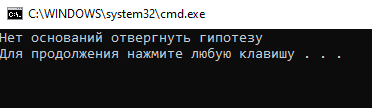
\includegraphics{img2.png} % Example image
	\caption{Проверка}
\end{figure}

\section{Исходный код}

Обычный текст вместо исходного кода
	
	
\section{Лишняя секция}


\section{Выводы}

Из результатов работы программ можно сказать, что гипотеза о том, что исследуемая случайная величина распределена по нормальному закону с математическим ожиданием 3.1 и стандартном квадратичном отклонении 1.667 принимается. 
 
Проверена гипотеза о соответствии распределения экспериментальных данных нормальному закону. Изучен критерий Хи-квадрат (критерия Пирсона) и его реализаций в Matlab и Python.

\end{document}